\section{First Algorithmic Approach}
The first algorithmic approach to find the boundary-defining Hamiltonian cycle of a square lattice graph is strongly related to the proof of Theorem~\ref{FourCornerLemma}. By assuming that the westernmost vertex of the northernmost vertices always has exactly two edges rightward and downward. 
\begin{enumerate}[1.]
\item Let $G_{x,y}$ be the direction to which the tile at $(x,y)$ points to. Set all $G_{x,y}=-1$, for $x,y \in \mathbb{Z}$
\item Set $x\gets x_0, y\gets y_0$, of the coordinates $x_0,y_0$ of the westernmost vertex of the northernmost vertices of graph $G$, $directions$ = $\{up,right,down,left\}$, $lastDirection\gets down$
\item \label{loopBegin} Set $direction \gets lastDirection+1 \pmod{4}$
\item $x'$ \gets ApplyDirection($x$, $direction$), $y'$ \gets ApplyDirection($y$, $direction$)
\item if not TileAt($x'$,$y'$) or $direction = lastDirection$ or $G_{x,y}\ne -1$, go to step $\ref{loopUpdate}$
\item Set $G_{x,y} = direction$, $x \gets x', y \gets y'$, $lastDirection \gets OppositeDirection(direction)$; go to step $\ref{loopBegin}$
\item \label{loopUpdate} $direction \gets direction+1 \pmod{4}$
\item if $direction\leq 3$, go to step $\ref{loopBegin}$
\item Stop.
\end{enumerate}
\begin{figure}[H]
\centering
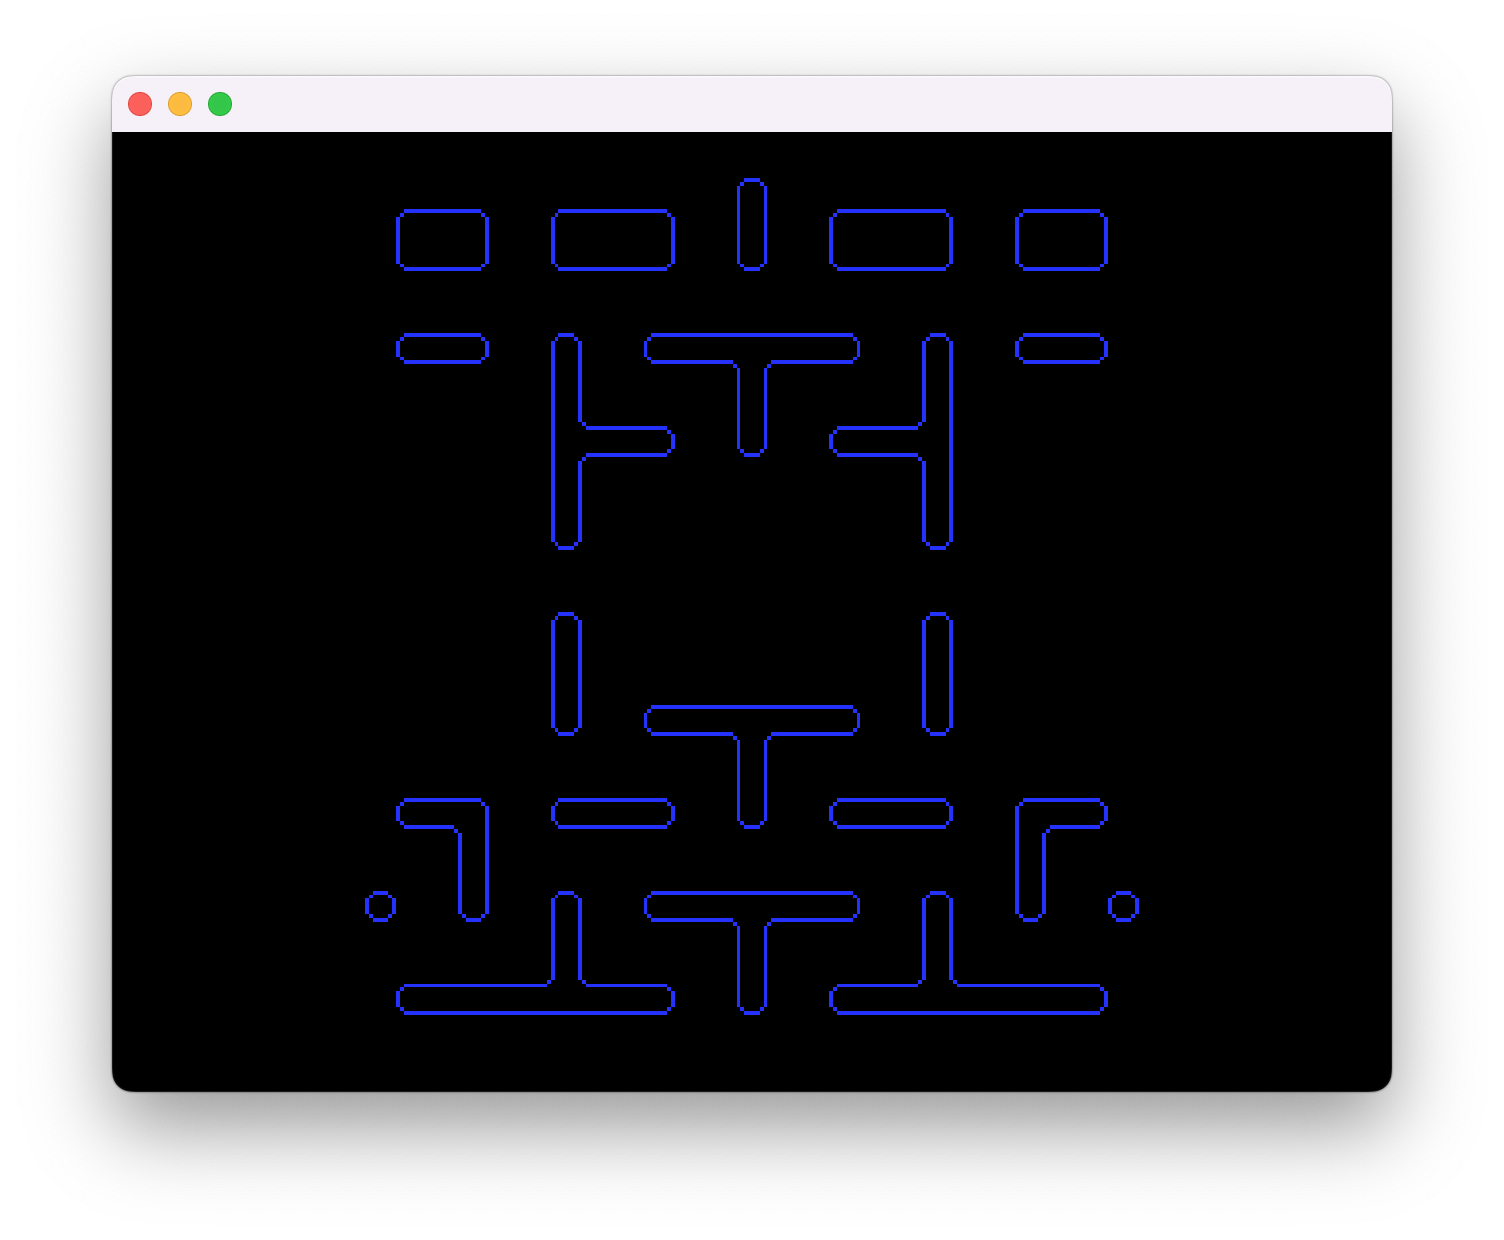
\includegraphics[width=0.8\linewidth]{Image-8.png}
\caption {Output of first algorithm\autocite{myself}}\label{FirstOutput}
\end{figure}